\documentclass[twoside]{book}

% Packages required by doxygen
\usepackage{fixltx2e}
\usepackage{calc}
\usepackage{doxygen}
\usepackage[export]{adjustbox} % also loads graphicx
\usepackage{graphicx}
\usepackage[utf8]{inputenc}
\usepackage{makeidx}
\usepackage{multicol}
\usepackage{multirow}
\PassOptionsToPackage{warn}{textcomp}
\usepackage{textcomp}
\usepackage[nointegrals]{wasysym}
\usepackage[table]{xcolor}

% Font selection
\usepackage[T1]{fontenc}
\usepackage[scaled=.90]{helvet}
\usepackage{courier}
\usepackage{amssymb}
\usepackage{sectsty}
\renewcommand{\familydefault}{\sfdefault}
\allsectionsfont{%
  \fontseries{bc}\selectfont%
  \color{darkgray}%
}
\renewcommand{\DoxyLabelFont}{%
  \fontseries{bc}\selectfont%
  \color{darkgray}%
}
\newcommand{\+}{\discretionary{\mbox{\scriptsize$\hookleftarrow$}}{}{}}

% Page & text layout
\usepackage{geometry}
\geometry{%
  a4paper,%
  top=2.5cm,%
  bottom=2.5cm,%
  left=2.5cm,%
  right=2.5cm%
}
\tolerance=750
\hfuzz=15pt
\hbadness=750
\setlength{\emergencystretch}{15pt}
\setlength{\parindent}{0cm}
\setlength{\parskip}{0.2cm}
\makeatletter
\renewcommand{\paragraph}{%
  \@startsection{paragraph}{4}{0ex}{-1.0ex}{1.0ex}{%
    \normalfont\normalsize\bfseries\SS@parafont%
  }%
}
\renewcommand{\subparagraph}{%
  \@startsection{subparagraph}{5}{0ex}{-1.0ex}{1.0ex}{%
    \normalfont\normalsize\bfseries\SS@subparafont%
  }%
}
\makeatother

% Headers & footers
\usepackage{fancyhdr}
\pagestyle{fancyplain}
\fancyhead[LE]{\fancyplain{}{\bfseries\thepage}}
\fancyhead[CE]{\fancyplain{}{}}
\fancyhead[RE]{\fancyplain{}{\bfseries\leftmark}}
\fancyhead[LO]{\fancyplain{}{\bfseries\rightmark}}
\fancyhead[CO]{\fancyplain{}{}}
\fancyhead[RO]{\fancyplain{}{\bfseries\thepage}}
\fancyfoot[LE]{\fancyplain{}{}}
\fancyfoot[CE]{\fancyplain{}{}}
\fancyfoot[RE]{\fancyplain{}{\bfseries\scriptsize Generated on Sun Dec 6 2015 21\+:43\+:17 for My Project by Doxygen }}
\fancyfoot[LO]{\fancyplain{}{\bfseries\scriptsize Generated on Sun Dec 6 2015 21\+:43\+:17 for My Project by Doxygen }}
\fancyfoot[CO]{\fancyplain{}{}}
\fancyfoot[RO]{\fancyplain{}{}}
\renewcommand{\footrulewidth}{0.4pt}
\renewcommand{\chaptermark}[1]{%
  \markboth{#1}{}%
}
\renewcommand{\sectionmark}[1]{%
  \markright{\thesection\ #1}%
}

% Indices & bibliography
\usepackage{natbib}
\usepackage[titles]{tocloft}
\setcounter{tocdepth}{3}
\setcounter{secnumdepth}{5}
\makeindex

% Hyperlinks (required, but should be loaded last)
\usepackage{ifpdf}
\ifpdf
  \usepackage[pdftex,pagebackref=true]{hyperref}
\else
  \usepackage[ps2pdf,pagebackref=true]{hyperref}
\fi
\hypersetup{%
  colorlinks=true,%
  linkcolor=blue,%
  citecolor=blue,%
  unicode%
}

% Custom commands
\newcommand{\clearemptydoublepage}{%
  \newpage{\pagestyle{empty}\cleardoublepage}%
}


%===== C O N T E N T S =====

\begin{document}

% Titlepage & ToC
\hypersetup{pageanchor=false,
             bookmarks=true,
             bookmarksnumbered=true,
             pdfencoding=unicode
            }
\pagenumbering{roman}
\begin{titlepage}
\vspace*{7cm}
\begin{center}%
{\Large My Project }\\
\vspace*{1cm}
{\large Generated by Doxygen 1.8.10}\\
\vspace*{0.5cm}
{\small Sun Dec 6 2015 21:43:17}\\
\end{center}
\end{titlepage}
\clearemptydoublepage
\tableofcontents
\clearemptydoublepage
\pagenumbering{arabic}
\hypersetup{pageanchor=true}

%--- Begin generated contents ---
\chapter{Main Page}
\label{index}\hypertarget{index}{}Este é o Subplayer. Um player de video baseado em Qt que funciona com os codecs que você já tenha instalado no seu computador 
\chapter{Hierarchical Index}
\section{Class Hierarchy}
This inheritance list is sorted roughly, but not completely, alphabetically\+:\begin{DoxyCompactList}
\item Q\+Main\+Window\begin{DoxyCompactList}
\item \contentsline{section}{Main\+Window}{\pageref{classMainWindow}}{}
\end{DoxyCompactList}
\item \contentsline{section}{subtitle}{\pageref{structsubtitle}}{}
\item \contentsline{section}{time\+Range}{\pageref{structtimeRange}}{}
\end{DoxyCompactList}

\chapter{Class Index}
\section{Class List}
Here are the classes, structs, unions and interfaces with brief descriptions\+:\begin{DoxyCompactList}
\item\contentsline{section}{\hyperlink{classMainWindow}{Main\+Window} \\*A \hyperlink{classMainWindow}{Main\+Window} class e a classe principal do programa, responsável por tocar o vídeo e organizar as legendas }{\pageref{classMainWindow}}{}
\item\contentsline{section}{\hyperlink{structsubtitle}{subtitle} \\*Esta subtitle struct é utilizada na contrução de uma estrutura de dados para representar as legendas }{\pageref{structsubtitle}}{}
\item\contentsline{section}{\hyperlink{structtimeRange}{time\+Range} \\*Esta \hyperlink{structtimeRange}{time\+Range} struct auxilia na definição de intervalos para cada legenda encontrada no arquivo }{\pageref{structtimeRange}}{}
\end{DoxyCompactList}

\chapter{File Index}
\section{File List}
Here is a list of all documented files with brief descriptions\+:\begin{DoxyCompactList}
\item\contentsline{section}{\hyperlink{mainwindow_8h}{mainwindow.\+h} \\*Este é o Subplayer. Um player de video para linux baseado em Qt que funciona com os codecs que você já tenha instalado no seu computador e te ajudar a aprender linguas estrangeiras }{\pageref{mainwindow_8h}}{}
\end{DoxyCompactList}

\chapter{Class Documentation}
\hypertarget{classMainWindow}{}\section{Main\+Window Class Reference}
\label{classMainWindow}\index{Main\+Window@{Main\+Window}}


A \hyperlink{classMainWindow}{Main\+Window} class e a classe principal do programa, responsável por tocar o vídeo e organizar as legendas.  




{\ttfamily \#include $<$mainwindow.\+h$>$}

Inheritance diagram for Main\+Window\+:\begin{figure}[H]
\begin{center}
\leavevmode
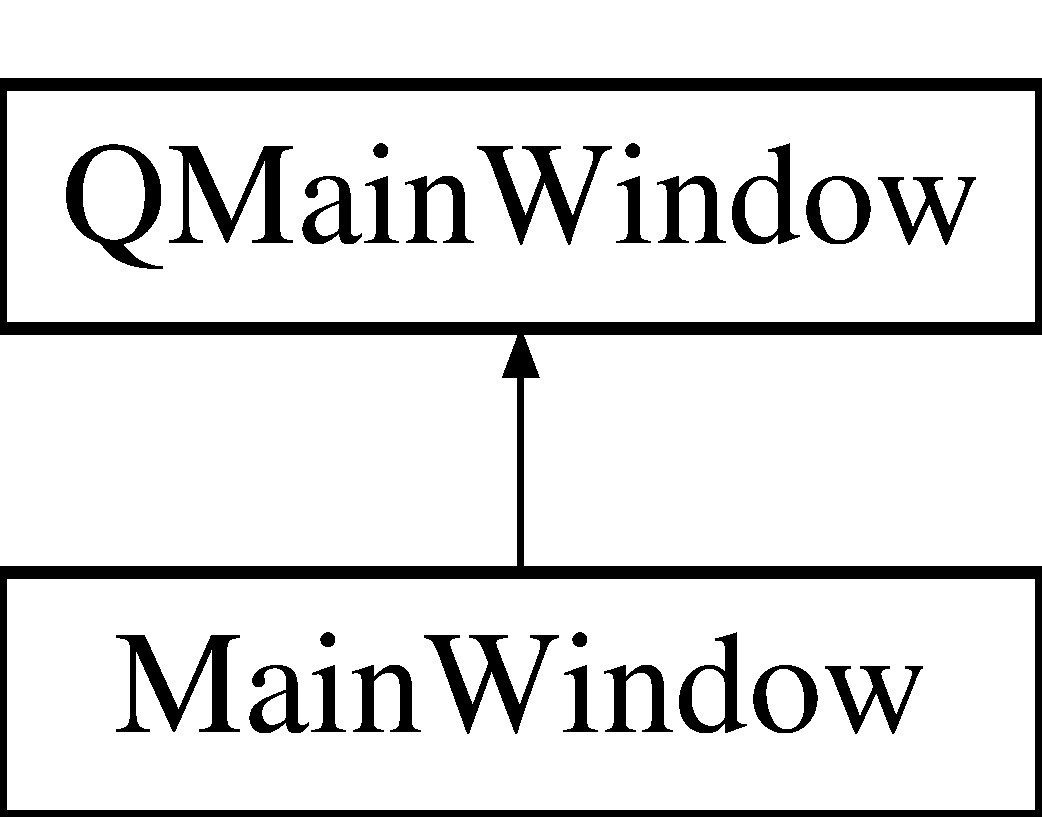
\includegraphics[height=2.000000cm]{classMainWindow}
\end{center}
\end{figure}
\subsection*{Public Member Functions}
\begin{DoxyCompactItemize}
\item 
\hypertarget{classMainWindow_a8b244be8b7b7db1b08de2a2acb9409db}{}{\bfseries Main\+Window} (Q\+Widget $\ast$parent=0)\label{classMainWindow_a8b244be8b7b7db1b08de2a2acb9409db}

\end{DoxyCompactItemize}
\subsection*{Protected Member Functions}
\begin{DoxyCompactItemize}
\item 
void \hyperlink{classMainWindow_abc2fe19d0ae9507b0b3f5dfa7e6e0fea}{design\+Main\+Window} ()
\begin{DoxyCompactList}\small\item\em Cria os componentes da tela principal. \end{DoxyCompactList}\item 
void \hyperlink{classMainWindow_a03799692902ab88a551b4dca1fa042db}{create\+Menu} ()
\begin{DoxyCompactList}\small\item\em Cria o menu principal. \end{DoxyCompactList}\item 
\hyperlink{structtimeRange}{time\+Range} \hyperlink{classMainWindow_a79cc6f131a72ba24e71ca6143e175726}{get\+Milisec\+Duration} (string duration)
\begin{DoxyCompactList}\small\item\em Retorna duração em milisegundos. \end{DoxyCompactList}\item 
list$<$ \hyperlink{structsubtitle}{subtitle} $\ast$ $>$ \hyperlink{classMainWindow_adf409fa41443eebae1afbe6b26746179}{getsubtitles} (string path)
\begin{DoxyCompactList}\small\item\em Cria lista que representa a legenda. \end{DoxyCompactList}\item 
vector$<$ Q\+String $>$ \hyperlink{classMainWindow_a0379a5ad1b2b9faaf543bae96d1bf479}{get\+String\+List} (string line)
\begin{DoxyCompactList}\small\item\em Retorna a lista de strings de uma linha da legenda. \end{DoxyCompactList}\item 
void \hyperlink{classMainWindow_ae12f8f63791595567b6250f8bb002bda}{resize\+Event} (Q\+Resize\+Event $\ast$event)
\begin{DoxyCompactList}\small\item\em Redimensiona a tela de video. \end{DoxyCompactList}\end{DoxyCompactItemize}
\subsection*{Protected Attributes}
\begin{DoxyCompactItemize}
\item 
Ui\+::\+Main\+Window $\ast$ \hyperlink{classMainWindow_a35466a70ed47252a0191168126a352a5}{ui}
\item 
\hypertarget{classMainWindow_af3f32d4111cefe576b4789f3611e99e8}{}Q\+Media\+Player $\ast$ {\bfseries player}\label{classMainWindow_af3f32d4111cefe576b4789f3611e99e8}

\item 
\hypertarget{classMainWindow_a063e8029e7ce646ef1bcdf84beb4157a}{}Q\+Main\+Window $\ast$ {\bfseries subwindow} = N\+U\+L\+L\label{classMainWindow_a063e8029e7ce646ef1bcdf84beb4157a}

\item 
\hypertarget{classMainWindow_a1673c9d0d60ad3586c8c64ab215b6089}{}Q\+Web\+View $\ast$ {\bfseries webview}\label{classMainWindow_a1673c9d0d60ad3586c8c64ab215b6089}

\item 
\hypertarget{classMainWindow_a3d44e16270b2e68a86399911f2704c10}{}int {\bfseries video\+Height}\label{classMainWindow_a3d44e16270b2e68a86399911f2704c10}

\item 
\hypertarget{classMainWindow_ae53e754f06ce9bc859e44e48d717454e}{}int {\bfseries video\+Width}\label{classMainWindow_ae53e754f06ce9bc859e44e48d717454e}

\item 
\hypertarget{classMainWindow_a864558ff87b64a491d601b9b2e31df0b}{}Q\+Video\+Widget $\ast$ {\bfseries video\+Widget}\label{classMainWindow_a864558ff87b64a491d601b9b2e31df0b}

\item 
\hypertarget{classMainWindow_a8d0199acb41711efb652ffeb569da73e}{}Q\+Grid\+Layout $\ast$ {\bfseries video\+Layout}\label{classMainWindow_a8d0199acb41711efb652ffeb569da73e}

\item 
\hypertarget{classMainWindow_a78fa3441fc4a50be4308d1184f86b7b3}{}Q\+V\+Box\+Layout $\ast$ {\bfseries subtitle\+Layout}\label{classMainWindow_a78fa3441fc4a50be4308d1184f86b7b3}

\item 
\hypertarget{classMainWindow_ad3bde47a75b6c59146d6aff1752d077f}{}Q\+Widget $\ast$ {\bfseries central\+Widget}\label{classMainWindow_ad3bde47a75b6c59146d6aff1752d077f}

\item 
\hypertarget{classMainWindow_a250010d22bbd4c7727b5af5b8e555f0d}{}Q\+Graphics\+Video\+Item $\ast$ {\bfseries video\+Item}\label{classMainWindow_a250010d22bbd4c7727b5af5b8e555f0d}

\item 
\hypertarget{classMainWindow_a51ac2b126495216832501cea3929c6f6}{}Q\+Graphics\+Scene $\ast$ {\bfseries scene}\label{classMainWindow_a51ac2b126495216832501cea3929c6f6}

\item 
\hypertarget{classMainWindow_a2ae234c8fc9c4a897231f2ead4ad6d29}{}Q\+Graphics\+View $\ast$ {\bfseries graphics\+View}\label{classMainWindow_a2ae234c8fc9c4a897231f2ead4ad6d29}

\item 
\hypertarget{classMainWindow_a5e98a81ef43bd540b7e23e5fcc6b8691}{}list$<$ \hyperlink{structsubtitle}{subtitle} $\ast$ $>$ \hyperlink{classMainWindow_a5e98a81ef43bd540b7e23e5fcc6b8691}{mysubs}\label{classMainWindow_a5e98a81ef43bd540b7e23e5fcc6b8691}

\begin{DoxyCompactList}\small\item\em Lista de legendas. \end{DoxyCompactList}\item 
\hypertarget{classMainWindow_a426da48f6e2f865b07a28533c07c4f7a}{}Q\+Menu $\ast$ {\bfseries file\+Menu}\label{classMainWindow_a426da48f6e2f865b07a28533c07c4f7a}

\item 
\hypertarget{classMainWindow_a74bc8963da39088cff8fcacdfedc1790}{}Q\+Action $\ast$ {\bfseries open\+File}\label{classMainWindow_a74bc8963da39088cff8fcacdfedc1790}

\item 
\hypertarget{classMainWindow_a0077cf8061006bfa6cf3772d7baea6e5}{}Q\+Push\+Button $\ast$ {\bfseries play\+Pause\+Button}\label{classMainWindow_a0077cf8061006bfa6cf3772d7baea6e5}

\item 
\hypertarget{classMainWindow_a2060b73304f4619b507ba3b0c985caad}{}Q\+Push\+Button $\ast$ {\bfseries stop\+Button}\label{classMainWindow_a2060b73304f4619b507ba3b0c985caad}

\item 
\hypertarget{classMainWindow_addc644fda913a37aa2e69ea2961a0424}{}Q\+Slider $\ast$ {\bfseries progress\+Slider}\label{classMainWindow_addc644fda913a37aa2e69ea2961a0424}

\item 
\hypertarget{classMainWindow_aed770176c46d1d2de1b45deeea185d19}{}Q\+Timer $\ast$ \hyperlink{classMainWindow_aed770176c46d1d2de1b45deeea185d19}{subtitle\+Timer}\label{classMainWindow_aed770176c46d1d2de1b45deeea185d19}

\begin{DoxyCompactList}\small\item\em Temporizador das legendas. \end{DoxyCompactList}\item 
\hypertarget{classMainWindow_a53fd1e1d3acbd985e622f97003c20e4e}{}Q\+String {\bfseries filename}\label{classMainWindow_a53fd1e1d3acbd985e622f97003c20e4e}

\item 
\hypertarget{classMainWindow_ade1a837c23e15bad80217a55b044ef27}{}Q\+String {\bfseries subtitle\+Name}\label{classMainWindow_ade1a837c23e15bad80217a55b044ef27}

\end{DoxyCompactItemize}


\subsection{Detailed Description}
A \hyperlink{classMainWindow}{Main\+Window} class e a classe principal do programa, responsável por tocar o vídeo e organizar as legendas. 

\subsection{Member Function Documentation}
\hypertarget{classMainWindow_a03799692902ab88a551b4dca1fa042db}{}\index{Main\+Window@{Main\+Window}!create\+Menu@{create\+Menu}}
\index{create\+Menu@{create\+Menu}!Main\+Window@{Main\+Window}}
\subsubsection[{create\+Menu()}]{\setlength{\rightskip}{0pt plus 5cm}void Main\+Window\+::create\+Menu (
\begin{DoxyParamCaption}
{}
\end{DoxyParamCaption}
)\hspace{0.3cm}{\ttfamily [protected]}}\label{classMainWindow_a03799692902ab88a551b4dca1fa042db}


Cria o menu principal. 

Essa funcao cria o menu principal do programa \begin{DoxyReturn}{Returns}
void 
\end{DoxyReturn}
\hypertarget{classMainWindow_abc2fe19d0ae9507b0b3f5dfa7e6e0fea}{}\index{Main\+Window@{Main\+Window}!design\+Main\+Window@{design\+Main\+Window}}
\index{design\+Main\+Window@{design\+Main\+Window}!Main\+Window@{Main\+Window}}
\subsubsection[{design\+Main\+Window()}]{\setlength{\rightskip}{0pt plus 5cm}void Main\+Window\+::design\+Main\+Window (
\begin{DoxyParamCaption}
{}
\end{DoxyParamCaption}
)\hspace{0.3cm}{\ttfamily [protected]}}\label{classMainWindow_abc2fe19d0ae9507b0b3f5dfa7e6e0fea}


Cria os componentes da tela principal. 

Essa funcao criar os componentes que compoem a tela principal \begin{DoxyReturn}{Returns}
void 
\end{DoxyReturn}
\hypertarget{classMainWindow_a79cc6f131a72ba24e71ca6143e175726}{}\index{Main\+Window@{Main\+Window}!get\+Milisec\+Duration@{get\+Milisec\+Duration}}
\index{get\+Milisec\+Duration@{get\+Milisec\+Duration}!Main\+Window@{Main\+Window}}
\subsubsection[{get\+Milisec\+Duration(string duration)}]{\setlength{\rightskip}{0pt plus 5cm}{\bf time\+Range} Main\+Window\+::get\+Milisec\+Duration (
\begin{DoxyParamCaption}
\item[{string}]{duration}
\end{DoxyParamCaption}
)\hspace{0.3cm}{\ttfamily [protected]}}\label{classMainWindow_a79cc6f131a72ba24e71ca6143e175726}


Retorna duração em milisegundos. 

Essa funçao calcula a duraçao em milisegundos de um a string do formato hh\+:mm\+:ss,sss-\/$>$hh\+:mm\+:ss,sss \begin{DoxyReturn}{Returns}
\hyperlink{structtimeRange}{time\+Range} 
\end{DoxyReturn}

\begin{DoxyParams}{Parameters}
{\em duration} & string contendo a duraçao. \\
\hline
\end{DoxyParams}
\begin{DoxyPrecond}{Precondition}

\begin{DoxyEnumerate}
\item duration no formato hh\+:mm\+:ss,sss-\/$>$hh\+:mm\+:ss,sss. 
\end{DoxyEnumerate}
\end{DoxyPrecond}
\hypertarget{classMainWindow_a0379a5ad1b2b9faaf543bae96d1bf479}{}\index{Main\+Window@{Main\+Window}!get\+String\+List@{get\+String\+List}}
\index{get\+String\+List@{get\+String\+List}!Main\+Window@{Main\+Window}}
\subsubsection[{get\+String\+List(string line)}]{\setlength{\rightskip}{0pt plus 5cm}vector$<$ Q\+String $>$ Main\+Window\+::get\+String\+List (
\begin{DoxyParamCaption}
\item[{string}]{line}
\end{DoxyParamCaption}
)\hspace{0.3cm}{\ttfamily [protected]}}\label{classMainWindow_a0379a5ad1b2b9faaf543bae96d1bf479}


Retorna a lista de strings de uma linha da legenda. 

essa função recebe uma string line que contém as palavras e retorna uma lista com cada string que representa as palavras da legenda. \begin{DoxyReturn}{Returns}
list$<$subtitle$\ast$$>$ 
\end{DoxyReturn}

\begin{DoxyParams}{Parameters}
{\em line} & linha de cada legenda \\
\hline
\end{DoxyParams}
\hypertarget{classMainWindow_adf409fa41443eebae1afbe6b26746179}{}\index{Main\+Window@{Main\+Window}!getsubtitles@{getsubtitles}}
\index{getsubtitles@{getsubtitles}!Main\+Window@{Main\+Window}}
\subsubsection[{getsubtitles(string path)}]{\setlength{\rightskip}{0pt plus 5cm}list$<$ {\bf subtitle} $\ast$ $>$ Main\+Window\+::getsubtitles (
\begin{DoxyParamCaption}
\item[{string}]{path}
\end{DoxyParamCaption}
)\hspace{0.3cm}{\ttfamily [protected]}}\label{classMainWindow_adf409fa41443eebae1afbe6b26746179}


Cria lista que representa a legenda. 

Essa funçao cria a lista que será utilizada para exibir as legendas no video \begin{DoxyReturn}{Returns}
list$<$subtitle$\ast$$>$ 
\end{DoxyReturn}

\begin{DoxyParams}{Parameters}
{\em path} & caminho para o arquivo da legenda \\
\hline
\end{DoxyParams}
\hypertarget{classMainWindow_ae12f8f63791595567b6250f8bb002bda}{}\index{Main\+Window@{Main\+Window}!resize\+Event@{resize\+Event}}
\index{resize\+Event@{resize\+Event}!Main\+Window@{Main\+Window}}
\subsubsection[{resize\+Event(\+Q\+Resize\+Event $\ast$event)}]{\setlength{\rightskip}{0pt plus 5cm}void Main\+Window\+::resize\+Event (
\begin{DoxyParamCaption}
\item[{Q\+Resize\+Event $\ast$}]{event}
\end{DoxyParamCaption}
)\hspace{0.3cm}{\ttfamily [protected]}}\label{classMainWindow_ae12f8f63791595567b6250f8bb002bda}


Redimensiona a tela de video. 

Essa funçao redimensiona a tela de video quando o usuário redimensionar a \hyperlink{classMainWindow}{Main\+Window} \begin{DoxyReturn}{Returns}
void 
\end{DoxyReturn}

\begin{DoxyParams}{Parameters}
{\em event} & evento de chamada \\
\hline
\end{DoxyParams}


\subsection{Member Data Documentation}
\hypertarget{classMainWindow_a35466a70ed47252a0191168126a352a5}{}\index{Main\+Window@{Main\+Window}!ui@{ui}}
\index{ui@{ui}!Main\+Window@{Main\+Window}}
\subsubsection[{ui}]{\setlength{\rightskip}{0pt plus 5cm}Ui\+::\+Main\+Window$\ast$ Main\+Window\+::ui\hspace{0.3cm}{\ttfamily [protected]}}\label{classMainWindow_a35466a70ed47252a0191168126a352a5}
E\+S\+S\+A\+S F\+U\+N\+CǑ\+E\+S E O\+B\+J\+E\+T\+O\+S D\+E\+V\+E\+R\+I\+A\+M S\+E\+R P\+R\+I\+V\+A\+T\+E, P\+O\+R\+E\+M P\+A\+R\+A F\+I\+N\+S D\+E D\+O\+C\+U\+M\+E\+N\+T\+A\+C\+A\+O S\+E\+R\+A\+O C\+O\+N\+S\+I\+D\+E\+R\+A\+D\+O\+S P\+R\+O\+T\+E\+C\+T\+E\+D. 

The documentation for this class was generated from the following files\+:\begin{DoxyCompactItemize}
\item 
\hyperlink{mainwindow_8h}{mainwindow.\+h}\item 
mainwindow.\+cpp\end{DoxyCompactItemize}

\hypertarget{structsubtitle}{}\section{subtitle Struct Reference}
\label{structsubtitle}\index{subtitle@{subtitle}}


Esta subtitle struct é utilizada na contrução de uma estrutura de dados para representar as legendas.  




{\ttfamily \#include $<$mainwindow.\+h$>$}

\subsection*{Public Attributes}
\begin{DoxyCompactItemize}
\item 
bool \hyperlink{structsubtitle_a12b5d59da640a60de07892449a14b06a}{played}
\item 
\hyperlink{structtimeRange}{time\+Range} \hyperlink{structsubtitle_ae3c12c11840733f601353d28bad10b26}{timerange}
\item 
vector$<$ vector$<$ Q\+String $>$ $>$ \hyperlink{structsubtitle_a8ea20b5e81c5028fb612ecb13183cb28}{firstline}
\end{DoxyCompactItemize}


\subsection{Detailed Description}
Esta subtitle struct é utilizada na contrução de uma estrutura de dados para representar as legendas. 

\subsection{Member Data Documentation}
\hypertarget{structsubtitle_a8ea20b5e81c5028fb612ecb13183cb28}{}\index{subtitle@{subtitle}!firstline@{firstline}}
\index{firstline@{firstline}!subtitle@{subtitle}}
\subsubsection[{firstline}]{\setlength{\rightskip}{0pt plus 5cm}vector$<$vector$<$Q\+String$>$ $>$ subtitle\+::firstline}\label{structsubtitle_a8ea20b5e81c5028fb612ecb13183cb28}
Armazena as Strings que compoem a legenda \hypertarget{structsubtitle_a12b5d59da640a60de07892449a14b06a}{}\index{subtitle@{subtitle}!played@{played}}
\index{played@{played}!subtitle@{subtitle}}
\subsubsection[{played}]{\setlength{\rightskip}{0pt plus 5cm}bool subtitle\+::played}\label{structsubtitle_a12b5d59da640a60de07892449a14b06a}
Indica se a legenda já foi tocada ou nao \hypertarget{structsubtitle_ae3c12c11840733f601353d28bad10b26}{}\index{subtitle@{subtitle}!timerange@{timerange}}
\index{timerange@{timerange}!subtitle@{subtitle}}
\subsubsection[{timerange}]{\setlength{\rightskip}{0pt plus 5cm}{\bf time\+Range} subtitle\+::timerange}\label{structsubtitle_ae3c12c11840733f601353d28bad10b26}
Tempo de inicio e final da legenda 

The documentation for this struct was generated from the following file\+:\begin{DoxyCompactItemize}
\item 
\hyperlink{mainwindow_8h}{mainwindow.\+h}\end{DoxyCompactItemize}

\hypertarget{structtimeRange}{}\section{time\+Range Struct Reference}
\label{structtimeRange}\index{time\+Range@{time\+Range}}


Esta \hyperlink{structtimeRange}{time\+Range} struct auxilia na definição de intervalos para cada legenda encontrada no arquivo.  




{\ttfamily \#include $<$mainwindow.\+h$>$}

\subsection*{Public Attributes}
\begin{DoxyCompactItemize}
\item 
qint64 \hyperlink{structtimeRange_a6155d9d43f5e0f233f5b69c4944585a2}{time\+Begin}
\item 
qint64 \hyperlink{structtimeRange_a289986776ea5e779100eb9ba782e8fd5}{time\+End}
\end{DoxyCompactItemize}


\subsection{Detailed Description}
Esta \hyperlink{structtimeRange}{time\+Range} struct auxilia na definição de intervalos para cada legenda encontrada no arquivo. 

\subsection{Member Data Documentation}
\hypertarget{structtimeRange_a6155d9d43f5e0f233f5b69c4944585a2}{}\index{time\+Range@{time\+Range}!time\+Begin@{time\+Begin}}
\index{time\+Begin@{time\+Begin}!time\+Range@{time\+Range}}
\subsubsection[{time\+Begin}]{\setlength{\rightskip}{0pt plus 5cm}qint64 time\+Range\+::time\+Begin}\label{structtimeRange_a6155d9d43f5e0f233f5b69c4944585a2}
Tempo de inicio da legenda \hypertarget{structtimeRange_a289986776ea5e779100eb9ba782e8fd5}{}\index{time\+Range@{time\+Range}!time\+End@{time\+End}}
\index{time\+End@{time\+End}!time\+Range@{time\+Range}}
\subsubsection[{time\+End}]{\setlength{\rightskip}{0pt plus 5cm}qint64 time\+Range\+::time\+End}\label{structtimeRange_a289986776ea5e779100eb9ba782e8fd5}
Tempo final da legenda 

The documentation for this struct was generated from the following file\+:\begin{DoxyCompactItemize}
\item 
\hyperlink{mainwindow_8h}{mainwindow.\+h}\end{DoxyCompactItemize}

\chapter{File Documentation}
\hypertarget{mainwindow_8h}{}\section{mainwindow.\+h File Reference}
\label{mainwindow_8h}\index{mainwindow.\+h@{mainwindow.\+h}}


Este é o Subplayer. Um player de video para linux baseado em Qt que funciona com os codecs que você já tenha instalado no seu computador e te ajudar a aprender linguas estrangeiras.  


{\ttfamily \#include $<$Q\+Main\+Window$>$}\\*
{\ttfamily \#include $<$Q\+Media\+Player$>$}\\*
{\ttfamily \#include $<$Q\+Video\+Widget$>$}\\*
{\ttfamily \#include $<$Q\+Debug$>$}\\*
{\ttfamily \#include $<$Qt\+Widgets$>$}\\*
{\ttfamily \#include $<$Q\+Graphics\+Video\+Item$>$}\\*
{\ttfamily \#include $<$Q\+Timer$>$}\\*
{\ttfamily \#include $<$vector$>$}\\*
{\ttfamily \#include $<$fstream$>$}\\*
{\ttfamily \#include $<$Q\+Box\+Layout$>$}\\*
{\ttfamily \#include $<$Q\+Media\+Meta\+Data$>$}\\*
{\ttfamily \#include $<$Q\+Web\+View$>$}\\*
{\ttfamily \#include $<$iostream$>$}\\*
{\ttfamily \#include $<$Q\+File\+Dialog$>$}\\*
\subsection*{Classes}
\begin{DoxyCompactItemize}
\item 
struct \hyperlink{structtimeRange}{time\+Range}
\begin{DoxyCompactList}\small\item\em Esta \hyperlink{structtimeRange}{time\+Range} struct auxilia na definição de intervalos para cada legenda encontrada no arquivo. \end{DoxyCompactList}\item 
struct \hyperlink{structsubtitle}{subtitle}
\begin{DoxyCompactList}\small\item\em Esta subtitle struct é utilizada na contrução de uma estrutura de dados para representar as legendas. \end{DoxyCompactList}\item 
class \hyperlink{classMainWindow}{Main\+Window}
\begin{DoxyCompactList}\small\item\em A \hyperlink{classMainWindow}{Main\+Window} class e a classe principal do programa, responsável por tocar o vídeo e organizar as legendas. \end{DoxyCompactList}\end{DoxyCompactItemize}


\subsection{Detailed Description}
Este é o Subplayer. Um player de video para linux baseado em Qt que funciona com os codecs que você já tenha instalado no seu computador e te ajudar a aprender linguas estrangeiras. 

\begin{DoxyAuthor}{Author}
Macedo\+:Igor 
\end{DoxyAuthor}
\begin{DoxyVersion}{Version}
Revision 1.\+1
\end{DoxyVersion}
Com o Subplayer, você pode tocar seus vídeos legendados e clicar em cada palavra da legenda para ter o significado tirado diretamente de um dicionário online. \begin{DoxyDate}{Date}
6 de Dezembro de 2015 
\end{DoxyDate}

%--- End generated contents ---

% Index
\backmatter
\newpage
\phantomsection
\clearemptydoublepage
\addcontentsline{toc}{chapter}{Index}
\printindex

\end{document}
